%----------------------------------------------------------------------
% Do's and Don'ts for scientific writing & presenting
% 
% Change history:
% * 06/2022 hp: Add contact details
% * 10/2021-11/2021 hp: v1.6 Refactor for public release
% * 03/2020 hp: v1.5 Add plagiarism examples
% * 02/2020 hp: v1.4 Add 'best practice for slide decks'
% * 02/2020 hp: v1.3 Add exemplary 'rendered bibliography items', add (redundant)
%                      caveats (which students seemed to overlook commonly)
% 
% * 11/2019 hp: v1.2 Added this year's common mistakes
% 
% * 09/2019 hp: v1.1 Change from EWA to VWA, simplify some passages
% 
% * 09/2018-10/2018 hp: v1.0 (added Peter's ``Typische aber vermeidbare
%                              Fehler, Stand 12.12.2017'')
% 
% * 11/2017-02/2018 hp: Initial draft
%----------------------------------------------------------------------
\documentclass[11pt,a4paper]{article}
\usepackage{styleguide}
%----------------------------------------------------------------------
% Your contact details
\author{
Horst Possegger\\[3mm]
{\small \texttt{possegger@icg.tugraz.at}}\\[3mm]
{\color{lgray}\scriptsize Insititute of Computer Graphics \& Vision\\[-1mm]
Graz University of Technology}
\and
Peter M. Roth\\[3mm]
{\small \texttt{Peter.M.Roth@vetmeduni.ac.at}}\\[3mm]
{\color{lgray}\scriptsize Institute for Computational Medicine\\[-1mm]
University of Veterinary Medicine Vienna}
}
%
% Title
\title{\goodstyle{Dos} and \badstyle{Don'ts} for\\[0.5em]Scientific Writing \& Presenting}
% 
% Version
% TODO 1.6 oder 1.0?
\version{1.6}

% TODOs
% * Version 1.6 oder 1.0 für erste public version?
% * Emails
% * cc-by-sa 4.0 ok?
% * intro double-check
% * literatur für presentations

\begin{document}
\tableofcontents
\pagebreak

\section{Introduction}
\label{sec-intro}
Scientific communication -- especially writing, but also presenting -- is a craft with a steep learning curve, as each and every student is about to learn.
The goal of this document is to accompany students on this ``climb'' and provide you the basics (helpful tipps \& recommendations) for writing your first scientific papers and presenting your work.
These recommendations focus on the Computer Science domain, although most are universally valid for other research fields, too.

Peter and Horst taught this craft for several years to their students at Graz University of Technology.
A preliminary version of this document accompanied our seminars -- \emph{``Introduction to Scientific Working''} and \emph{``Writing Scientific Papers''} (German: \emph{"Verfassen wissenschaftlicher Arbeiten"}) -- where students learned (1)~how to write scientific papers and (2)~how to prepare and give a scientific presentation. 

From our experience over the years, we summarized typical errors, so you can avoid them from the beginning.
Thus, we include the most important \goodstyle{dos} and \badstyle{dont's} to help you get started with scientific writing and presenting.
To this end, you should be aware of:
\begin{itemize}
\item How to cite papers correctly (Section~\ref{sec-references}).
\item What to (not) include in a bibliography (Section~\ref{sec-bibtex}).
\item Typesetting figures and tables correctly (Section~\ref{sec-figures}).
\item Mathematical writing (Section~\ref{sec-mathematics}).
\item Avoid plagiarism (Section~\ref{sec-plagiarism}).
\item Best practices for scientific presentations (Section~\ref{sec-presentations}).
\item General language-related advice (especially for non-native speakers) to get familiar with some specialities of scientific writing in English (Section~\ref{sec-writing}).
\end{itemize}

\subsubsection*{A Note on Typesetting:}
% In general, you can use any typesetting software to prepare your scientific papers (including office applications such as Microsoft Word or LibreOffice), as long as you adhere to the defined layout requirements (specified by the editor, conference chairs, \emph{etc.}).
We highly recommend using \LaTeX, as it simplifies layouting scientific texts a lot.
This includes the generation of bibliographies, correct and consistent citation, referring to figures, tables, or equations, and, in general, ensuring a consistent layout following the requested style. 

To help you get started with \LaTeX, this document provides several typesetting examples.
This, however, is not a step-by-step \LaTeX~tutorial.
If you have never used \LaTeX~before, you may want to check out a beginner's tutorial (\emph{e.g.} on \href{https://www.overleaf.com/learn/latex/Learn_LaTeX_in_30_minutes}{Overleaf}\footnote{Overleaf \LaTeX~tutorial: \url{https://www.overleaf.com/learn/latex/Learn_LaTeX_in_30_minutes}}) and refer to Q\&A sites, such as the great community site on \href{https://tex.stackexchange.com}{\TeX~-- \LaTeX~Stack Exchange}\footnote{\TeX~-- \LaTeX~Stack Exchange: \url{https://tex.stackexchange.com}}.

\newpage
\section{References \& Citations}
\label{sec-references}

Any content originating from others must be cited correctly in any document you will ever write, for several reasons:
\begin{enumerate}
  \item To support your own arguments by bringing them into context with existing works.
  \item To substantiate the credibility of your statements.
  \item To allow for traceability.
  \item To acknowledge their work.
\end{enumerate}
However, \textbf{pay attention to the quality of your references!}
There are many \emph{predatory journals and conferences} which do not follow scientific standards (even if they claim to have \emph{peer review}). As a \textbf{rule of thumb}, check for each reference you want to use:
\begin{enumerate}
  \item The \emph{journal and conference rankings} (\emph{e.g.} \href{https://scholar.google.com/citations?view_op=top_venues&hl=en&vq=eng}{Google Scholar}\footnote{Google Scholar rankings: \url{https://scholar.google.com/citations?view_op=top_venues&hl=en&vq=eng}}, \href{https://academic.microsoft.com/topic/41008148}{Microsoft Academic Search}\footnote{Microsoft Academic Search rankings: \url{https://academic.microsoft.com/topic/41008148}} or \href{https://aminer.org/ranks/conf}{ArnetMiner}\footnote{ArnetMiner rankings: \url{https://aminer.org/ranks/conf}}) to check whether the paper was published at a top tier journal/conference.
  \item The \emph{Journal Citation Reports (JCR) impact factor} of journals (which can be looked up at their official websites). 
  \item The \emph{citation count} of the corresponding paper and the scholarly metrics (\emph{e.g.} \emph{h-index} or \emph{i10-index}) of the author(s).
\end{enumerate}
As a \textbf{warm-up exercise}, look up the rankings and metrics/impact factors for (1)~the top tier computer vision \& machine learning conference \emph{IEEE/CVF Conference on Computer Vision and Pattern Recognition (CVPR)}, (2)~the top tier computer science journal \emph{IEEE Transactions on Pattern Analysis and Machine Intelligence (TPAMI)}, and (3)~the renowned multidisciplinary journal \emph{Nature}.

\subsubsection*{Direct Quotations:}
If you ever need to copy text directly, ensure that these \emph{direct quotations} are clearly made apparent \badstyle{to avoid plagiarism}.
This can be done by changing the layout to highlight the copied text passages. For example: use italicized fonts, quotation marks, and put the text in an indented block.
% 
For example, the Austrian Universitätsgesetz 2002~(UG) defines plagiarism as:
\begin{center}
\begin{minipage}{0.75\textwidth}
\emph{``Ein \textbf{Plagiat} liegt jedenfalls dann vor, wenn \textbf{Texte, Inhalte oder Ideen} übernommen und als eigene ausgegeben werden. Dies umfasst insbesondere die Aneignung und Verwendung von \textbf{Textpassagen, Theorien, Hypothesen, Erkenntnissen oder Daten} durch \badstyle{direkte, paraphrasierte oder übersetzte Übernahme} \textbf{ohne entsprechende Kenntlichmachung} und Zitierung der Quelle und der Urheberin oder des Urhebers.''} (UG §51, Z31)
\end{minipage}
\end{center}

Note, however, that computer science papers almost \textbf{never use direct quotations}.
Instead, we use \textbf{indirect quotations}, which means that content from others (algorithms, ideas, evaluations, data, \emph{etc.}) is only referred to or summarized in your own words.
For more details, refer to the plagiarism examples in Section~\ref{sec-plagiarism}.
% The following subsections present \goodstyle{best practice examples} and \badstyle{common mistakes} you should mind when writing your papers.
% To do this correctly, follow these guidelines:

\subsection{Referencing a Paper}
% Keep the following \goodstyle{best practice examples} and \badstyle{common mistakes} in mind when writing your papers.
\begin{itemize}
\item Whenever you mention a method \textbf{for the first time} in a document, cite the corresponding paper. For example, ``we use \goodstyle{SIFT~\nohrefcite{lowe04}} features to match corresponding points between image pairs''.

\item \textbf{Back your statements by references} -- if you say ``this is well known/this has been done before'', also list the relevant papers (those which have done ``this'' before or which have proposed ``this'').

\item References are \textbf{part of the sentence} -- thus, pay attention to correct punctuation: ``\goodstyle{[...]~poses and scales~[5].}`` instead of ``\badstyle{[...]~poses and scales. [5]}''.
 
\item Similarly, \textbf{never place a reference after a paragraph}. In scientific literature, this is not a correct citation (and additionally, does not indicate that you based the information within this paragraph on the corresponding paper).
 
\item There must be a single space between the text and the reference: ``\goodstyle{[...]~object detection{\textvisiblespace}[5]}'' instead of ``\badstyle{[...]~object detection[5]}'' or ``\badstyle{[...]~object detection{\textvisiblespace}{\textvisiblespace}[5]}''.
 
\item To cite a paper with \LaTeX, you need to have a bibliography entry (will be explained in Section~\ref{sec-bibtex}) and simply use the \texttt{\textbackslash{cite}\{\}} command. To prevent unwanted line breaks, always use a \emph{protected space} (special character '\texttt{$\sim$}')  instead of a standard space '\textvisiblespace' -- pay attention to the corresponding \LaTeX~sources of the following examples.
\end{itemize}
% 
\begin{goodexample}[Correct Citation of a Single Paper]
  \begin{NoHyper}
    According to Smith~\cite{smith14}, the quick brown fox jumped
over the lazy dog.

It is well known that the quick brown fox jumps over the lazy
dog~\cite{smith14}.

We apply Dijkstra's algorithm~\cite{dijkstra59} to find the
shortest path.

  
    \inlatex{examples/single_citation_good.tex}
  \end{NoHyper}
\end{goodexample}

\vspace{-1.5em}
\begin{badexample}[Incorrect Citation of a Single Paper]
  \begin{NoHyper}
    The lazy dog uses \badstyle{free-floating references.~\cite{smith14}}
    \vspace{0.25cm}
    
    There must always be a space between text and citation, \badstyle{not like 
    this\cite{roe17}}.
    \vspace{0.25cm}
    
    Pay attention not to add two spaces: in \LaTeX, ``\texttt{text{\textvisiblespace}$\sim${\textbackslash}cite\{dijkstra59\}}'' will incorrectly produce ``\badstyle{text{\textvisiblespace}{\textvisiblespace}\cite{dijkstra59}}''.
  \end{NoHyper}
\end{badexample}


\subsection{Referencing Multiple Papers at Once}

\begin{itemize}
  \item Sort multiple references in ascending order to improve readability. This helps your reader checking your references more efficiently.
  \item If you \textbf{cite multiple} papers at once, put them in a single citation -- in \LaTeX, you use a single \texttt{\textbackslash{cite}\{label1, label2, ...\}} command.
\end{itemize}

\begin{goodexample}[Correct Citation of Multiple Papers]
  \begin{NoHyper}
    This can be solved by~\cite{everyman14, roe17, smith14}.

Sorting references, such as~\cite{dijkstra59, everyman14, smith14},
speeds up the reading flow.

If you talk about \emph{much interest in/many works on} a topic, 
also list them, such as ``this topic has been explored by many
approaches, \emph{e.g.}~\cite{dijkstra59, roe17, smith14}''.

  
    \inlatex{examples/multiple_citations_good.tex}
  \end{NoHyper}
\end{goodexample}
\vspace{-1.5em}
\begin{badexample}[Incorrect Citation of Multiple Papers]
  \begin{NoHyper}
    This can be solved by \badstyle{\cite{everyman14}, \cite{lowe04}, \cite{smith14}}.

Maximize your reader's effort with unsorted references, such as~\badstyle{[17, 8, 42, 6, 99]}.

There are \badstyle{many algorithms} 
to solve this problem \badstyle{(But I don't list any)}.

  \end{NoHyper}
\end{badexample}



\subsection{Author Names and \emph{et al.}}
\label{sec-author-names-et-al}

\begin{itemize}
    \item If a paper is authored by three or more people, use \emph{et al.} This is an abbreviation of the Latin \emph{et alii}, meaning ``and others''.
    \item In a \emph{presentation}, \badstyle{never say ``Smith \emph{et al.}''} -- either say the full Latin form ``Smith \emph{et alii}'' or (even better) \goodstyle{say ``Smith and colleagues''}.
    \item If you refer to the authors of a paper, only use their surnames.
\end{itemize}

\begin{goodexample}[Correctly Referring to Authors]
  \begin{NoHyper}
    \begin{itemize}[leftmargin=1em]
        \item Single author: Smith~[4] proposed frobnication.
        
        \item Two authors: Roe and Doe~[3] extended this approach.
        
        \item Three or more: Everyman \emph{et al.}~[2] studied frobnicating machines.
    \end{itemize}

    \pagebreak

    {\normalsize\setstretch{1.2}
    \textbf{Bibliography of this Example:}
    \vspace{1em}
    
    {\normalsize
        \exemplarybibline{[2]}{R. Everyman, M. Major, J. Bloggs, and J. Roe. Can a Machine Frobnicate? In \emph{Proc. of the International Foo Filter Symposium}, 2014.}
        
        \exemplarybibline{[3]}{J. Roe and J. Doe. The Frobnicatable Foo Filter and its Applications. In \emph{Proc. of the Conference on Frobnication}, 2017.}
        
        \exemplarybibline{[4]}{J. Smith. Frobnication Tutorial. \emph{Journal of Theoretical Foo Filters}, 12(4):23--42, 2014.}
    }
    }
  \end{NoHyper}
\end{goodexample}

\begin{badexample}[Incorrectly Referring to Authors]
  \begin{NoHyper}
    \begin{itemize}[leftmargin=1em]
    \item ``\badstyle{Roe \emph{et al.}}~[3] proposed...'' is wrong, because there are only two authors: ``\goodstyle{Roe and Doe}~[3] proposed...''
        
    \item ``\badstyle{Everyman, Major, Bloggs, and Roe}~[2] showed...'' is wrong, because more than two authors requires \emph{et alii}: ``\goodstyle{Everyman, \emph{et al.}}~[2] showed...''
        
    \item ``\badstyle{Everyman, Major, \emph{et al.}}~[2]'' is also wrong, because we only write the first author's name when using \emph{et alii}: ``\goodstyle{Everyman, \emph{et al.}}~[2]''.
        
    \item ``\badstyle{J. Smith}~[4] showed...'' is wrong, because we should not include the author's first name: ``\goodstyle{Smith}~[4] showed...''
        
    \item ``Smith~[4] \badstyle{show}...'' is wrong, because a single author requires the \emph{third-person singular} form: ``Smith~[4] \goodstyle{shows}...''
    \end{itemize}
 
    % larger space as pagebreak does not work
    \vspace{2.0em}

    {\normalsize\setstretch{1.2}
    \textbf{Bibliography of this Example:}
    \vspace{1.0em}


    {\normalsize
        \exemplarybibline{[2]}{R. Everyman, M. Major, J. Bloggs, and J. Roe. Can a Machine Frobnicate? In \emph{Proc. of the International Foo Filter Symposium}, 2014.}
        
        \exemplarybibline{[3]}{J. Roe and J. Doe. The Frobnicatable Foo Filter and its Applications. In \emph{Proc. of the Conference on Frobnication}, 2017.}
        
        \exemplarybibline{[4]}{J. Smith. Frobnication Tutorial. \emph{Journal of Theoretical Foo Filters}, 12(4):23--42, 2014.}
    }
    }
  \end{NoHyper}
\end{badexample}




\newpage
\section{Bibliography}
\label{sec-bibtex}

In this section, we first summarize general recommendations for bibliographies (see Section~\ref{sec-bibtex-general}).
Then, we list exemplary bibliography entries showing the \textbf{required fields for different publication types} (such as papers, books, \emph{etc.}), along with their corresponding BibTeX entry (see Section~\ref{sec-bibtex-entries}) and provide suggestions that help you use BibTeX more efficiently (see Section~\ref{sec-bibtex-extras}).
Additionally, we demonstrate how to \textbf{correctly compile a PDF with \LaTeX+BibTeX} (see Section~\ref{sec-bibtex-compile}).


\subsection{General Recommendations for Bibliographies}
\label{sec-bibtex-general}

\begin{itemize}
\item \textbf{Never copy a bibliography entry} without double-checking it yourself (neither from the internet, nor from another paper's bibliography)! Unfortunately, many published papers (even from top tier conferences and high impact journals) contain sloppy and/or incorrect references. Similarly, references listed on Google Scholar, ResearchGate, \emph{etc.} are quite often incomplete. Thus, check every reference you want to add to your paper for:
% \item Thus, it is necessary to check every reference for
%
\vspace{-0.25cm}
%
\begin{itemize}
\item \textbf{Correctness} -- double-check your references, \emph{e.g.} by looking up the publication in the official conference proceedings or journal.
\item \textbf{Consistency} -- use the same abbreviations, the same name/style to refer to conferences or journals.
\item \textbf{Completeness} -- each reference must contain at least the following fields (more details for each publication type are provided in Section~\ref{sec-bibtex-entries}):
%
% \vspace{-0.25cm}
%
\begin{itemize}[label=$\bullet$]
\item Authors
\item Title
\item Source (conference, journal, book, \emph{etc.})
\item Issue/volume/number (for journal articles and technical reports)
\item Page numbers (for journal articles)
\item Year of publication
\end{itemize}
\end{itemize}

\item Each reference in your bibliography \textbf{must be cited at least once} within the text.

\item Avoid lexicographic entries (this usually happens if you copy the name of a conference/journal from some website). For example, compare the following:
%
\vspace{-0.25cm}
%
\begin{itemize}
\item Authors. Title. In \emph{Proc. of the \goodstyle{IEEE Conference on Computer Vision and Pattern Recognition}}, 2020.
\item Authors. Title. In \emph{Proc. of the \badstyle{Computer Vision and Pattern Recognition, IEEE Conference on}}, 2020.
\end{itemize}

\item Similarly, remove redundant information from the conference names, such as the year of publication (as this will be stated separately, as specified by the corresponding bibliography style).
%
\vspace{-0.25cm}
%
\begin{itemize}
\item Authors. Title. In \emph{Proc. of the \goodstyle{IEEE Intelligent Vehicles Symposium (IV)}}, 2019.
\item Authors. Title. In \emph{Proc. of the \badstyle{2019 IEEE Intelligent Vehicles Symposium (IV)}}, 2019.
\end{itemize}

\item For well-known conferences, no ordinal numbers are needed. This information can be
-- if anyone is actually interested in -- looked up easily online:
%
\vspace{-0.25cm}
%
\begin{itemize}
\item Authors. Title. In \emph{Proc. of the \goodstyle{International Conference on Frobnication}}, 2019.
\item Authors. Title. In \emph{Proc. of the \badstyle{23\textsuperscript{rd} International Conference on Frobnication}}, 2019.
\end{itemize}

\item Conference proceedings are usually digital. Thus, there is no need to include volume or pages (it is also surprisingly difficult to extract this information correctly)!

\end{itemize}


% \vfill
\subsection{Required Bibliography Fields}
\label{sec-bibtex-entries}

As mentioned above, depending on the publication type you want to cite (\emph{e.g.} conference papers, books, \emph{etc.}), there are different \textbf{required fields} you must provide in your bibliography. Below, you'll find examples for (almost) all publication types you'll need.
For each type, we list the required fields you have to provide in your bibliography (such as \texttt{title}, \texttt{author}, \emph{etc.}) within the corresponding exemplary BibTeX entry.
Also pay special attention to the additional notes/caveats as these summarize common mistakes you should avoid.

%% Conference
\bibtexample{Conference Paper}{examples/bibtex_proceedings.tex}{%
  \begin{itemize}
    \item[{[42]}] J. Doe and J.~J. Smith. A Solution to Foo. In \textit{Proceedings of the Conference on Scientific Writing}, 2021.
  \end{itemize}%
}{%
  \begin{itemize}
    \item You have to \textbf{explicitly write} ``\emph{Proceedings of the}'' or ``\emph{Proc. of the}'' inside the \texttt{booktitle} field.
    \item The extra curly braces (\emph{e.g.} \texttt{\{F\}oo}) within the \texttt{title} field ensure that the \textbf{capitalization} won't be changed by BibTeX.
    \item Conference proceedings are usually digital -- there is no need to include \emph{volume} or \emph{pages} (it's also surprisingly difficult to get this information correctly)!
    \item Ensure that you write the conference names correctly ordered -- if an online library uses lexicographic entries, \emph{e.g.} a conference name similar to \emph{``\badstyle{Scientific Writing, Conference on}''}, you have to correct this as \texttt{booktitle = \{Proceedings of the Conference on Scientific Writing\}}.
    \item Ordinal numbers should not be included in the conference name, \emph{e.g.} remove the ``\emph{23\textsuperscript{rd}}'' within ``\emph{\badstyle{23\textsuperscript{rd}} International Conference on Frobnication.}''
  \end{itemize}%
}

%% Journal
\bibtexample{Journal Article}{examples/bibtex_journal.tex}{%
  \begin{itemize}
    \item[{[23]}] Z. Kalal, K. Mikolajczyk, and J. Matas. Tracking-Learning-Detection. \textit{IEEE Transactions on Pattern Analysis and Machine Intelligence}, 34(7):1409--1422, 2012.
  \end{itemize}%
}{%
  \begin{itemize}
   \item \textbf{Always double-check} the \emph{volume} and \emph{number/issue} (some journals only publish \emph{volumes}).
   \item Use a \textbf{hyphen} (double dash) for the page range, \emph{i.e.} \texttt{pages = \{1409--1422\}}.
  \end{itemize}
}
\vfill


%% Book
\bibtexample{Book}{examples/bibtex_book.tex}{%
  \begin{itemize}
    \item[{[48]}] C.~M. Bishop. \textit{Pattern Recognition and Machine Learning}. Springer, first edition, 2006.
  \end{itemize}%
}{}

%% Book chapter
\bibtexample{Book Chapter}{examples/bibtex_bookchapter.tex}{%
  \begin{itemize}
    \item[{[49]}] C.~M. Bishop and J. Lasserre. \textit{Bayesian Statistics}, chapter \textit{Generative or Discriminative? Getting the Best of Both Worlds}, pages 3--24. Oxford University Press, 2007.
  \end{itemize}%
}{%
  \begin{itemize}
   \item Be aware that in this case the \textbf{\emph{title} field} is the \textbf{title of the
   book}, whereas the \textbf{\emph{chapter} field} is the name of the \textbf{actual
   contribution!}
  \end{itemize}
}


%% Thesis
\bibtexample{Thesis}{examples/bibtex_thesis.tex}{%
  \begin{itemize}
    \item[{[99]}] P. Fearnhead. \textit{Sequential Monte Carlo methods in filter theory}. PhD thesis, University of Oxford, Department of Statistics, 1998.
  \end{itemize}%
}{\begin{itemize}
    \item For a master's thesis, use the BibTeX entry type \texttt{@mscthesis} instead.
  \end{itemize}}

% \vfill
%% Technical Report, techreport
\bibtexample{Technical Report}{examples/bibtex_techreport.tex}{%
  \begin{itemize}
    \item[{[27]}] S. Nayar and Y. Nakagawa. \textit{Shape from Focus}. Technical Report CMU-RI-TR-89-27, Carnegie Mellon University, 1989.
  \end{itemize}%
}{}

%% arXiv
% @Peter: bitte aendern, falls dir mein arXiv Stil nicht passt
\bibtexample{Papers found on arXiv}{examples/bibtex_arxiv.tex}{%
  \begin{itemize}
    \item[{[99]}] H. Nam, M. Baek, and B. Han. Modeling and Propagating CNNs in a Tree Structure for Visual Tracking. \textit{arXiv CoRR}, abs/1608.07242, 2016. URL \texttt{https://arxiv.org/abs/1608.07242}.
  \end{itemize}%
}{\begin{itemize}
    \item \textbf{Double-check} (and then triple-check) \textbf{any arXiv content} -- are you really sure that the paper has not been published already at a conference/journal?
  \end{itemize}}

%% URLs
\bibtexample{URLs}{examples/bibtex_url.tex}{%
  \begin{itemize}
    \item[{[13]}] J.-Y. Bouguet. Camera Calibration Toolbox for Matlab. \texttt{http://www. vision.caltech.edu/bouguetj/calib\_doc/index.html}, 2010. Online; accessed July 30, 2017.
  \end{itemize}%
}{%
\begin{itemize}
  \item Use URLs in your bibliography \textbf{only if you really have to}, \emph{e.g.} when referring to a software toolbox or framework that you used.
  
  \item It is recommended that you place URL references within footnotes (\LaTeX: \lstinline[language={[LaTeX]TeX},basicstyle=\bfseries]{\\footnote\{\}}) instead of your bibliography.
   
\item URLs may contain characters with special meaning to \LaTeX/BibTeX, such as the underscore above. To prevent compilation errors, properly escape those characters, \emph{e.g.} use \texttt{'\textbackslash\_'} instead of a plain \texttt{'\_'}. The same also applies for the 
   $\sim$ symbol, which -- when copied from URLs -- would be incorrectly interpreted as
   protected space. Thus, you can use
   \lstinline[language={[LaTeX]TeX},basicstyle=\bfseries]{$\\sim$},
   \lstinline[language={[LaTeX]TeX},basicstyle=\bfseries]{\\texttildelow}, or
   \lstinline[language={[LaTeX]TeX},basicstyle=\bfseries]{\\~\{\}}
   instead. See Section~\ref{sec-spec:tex} on how to typeset special characters in \LaTeX.
\end{itemize}
}


% \vfill
\pagebreak
\subsection{BibTeX Best Practices}
\label{sec-bibtex-extras}
\begin{itemize}
\item To ensure that BibTeX-entries are shown correctly in the bibliography some
special formatting rules have to be followed:
% 
\bibtexampleplain{BibTeX Special Formatting Rules}{
\begin{itemize}[leftmargin=1em]
  \item Put extra curly braces within the \texttt{title} field to ensure that the capitalization won't be changed by BibTeX, \emph{e.g.} \texttt{title = \{\{T\}his is a \{C\}apitalized \{F\}oo\}}.

  \item Use the corresponding \LaTeX~commands to typeset \emph{diacritics} or \emph{umlauts}, \emph{e.g.} \texttt{\{\textbackslash{v}\{r\}\}} produces \v{r}, \texttt{\{\textbackslash"A\}} produces \"A, \texttt{\{\textbackslash'a\}} produces \'a, \emph{etc.} See also Section~\ref{sec-spec:tex} on how to typeset umlauts and diacritics in \LaTeX.

  \item Use double dashes for the page range, \emph{i.e.} \texttt{pages = \{1409--1422\}}. A single dash is reserved for compound words, \emph{e.g.} ``state-of-the-art''.
\end{itemize}}

\item BibTeX allows several ways to list the author names of a publication.
To ensure that first and surnames are always identified (and typeset) correctly, we recommend you use the following format:
% 
\bibtexample{BibTeX Author Names}{examples/bibtex_authors.tex}{}{}{}

\item Define BibTeX strings for conference/journal names. These are similar to constant variables or pre-processor defines and ensure that you use the corresponding conference/journal name consistently. Additionally, they simplify changing the name (\emph{e.g.} to fix a typo):
% 
\bibtexample{BibTeX Strings}{examples/bibtex_strings.tex}{}{}{}

\item Organize the labels of your bibliography entry such that you can easily recall the papers while writing: a label like \texttt{best-practices} may be easier to recall/remember than \texttt{dos-and-donts-for-scientific-writing-and-presenting}.\\You can also add arbitrary prefixes to create your own label taxonomy:
%
\bibtexample{BibTeX Labels}{examples/bibtex_labels.tex}{}{}{}

\end{itemize}

%
% \pagebreak
% \vfill
\subsection{Compile the Bibliography with BibTeX}
\label{sec-bibtex-compile}

You need to invoke your \LaTeX~compiler multiple times to ensure correct 
cross-referencing.
Assuming you use \texttt{pdflatex} (as your \LaTeX~compiler) and \texttt{bibtex} (as your BibTeX compiler), you need to run:
\begin{enumerate}
 
\item \texttt{pdflatex mypaper.tex}\\[.5em]
This first run yields a warning like ``\emph{There were undefined references}'' and your PDF will contain lots of ``[?]''.

\item \texttt{bibtex mypaper}\\[.5em]
BibTeX collects all bibliography entries you referred to in your document. From now on, all references should be known (unless there were some typos) -- so you need to re-compile your PDF.

\item \texttt{pdflatex mypaper.tex}\\[.5em]
This run yields a warning like ``\emph{References may have changed, rerun}'' indicating that the page numbers of some citations may have changed (due to replacing the previous ``[?]'' by the correct reference).

\item \texttt{pdflatex mypaper.tex}\\[.5em]
Done -- now you have your final PDF.

\end{enumerate}



\newpage
\section{Figures and Tables}
\label{sec-figures}
\begin{itemize}
\item Use figures and tables to \textbf{help the reader understand your work}. For example, they can provide an overview of your approach; a summary of your key findings; a comparison of different approaches/methodologies; \emph{etc.}
 
\item Pay attention to \textbf{correctly cite the source} of an illustration or table! Even if you just copied parts of an illustration/table, you still need to state this explicitly.
 
\item Whenever you include illustrations or tables within your documents, you must \textbf{refer to them within the corresponding text}, \emph{e.g.} ``\goodstyle{Fig.~1 illustrates}'' or ``\goodstyle{results are shown in Table~2}''.

\item With \LaTeX, you just need to \verb,\label{}, your figure or table and then refer to it using the \verb,\ref{}, command.
To prevent unwanted line breaks before the figure/table number, use the \emph{protected space} (\emph{i.e.} the tilde symbol, $\sim$) directly before \verb,\ref{},.
Check the examples within this section on how to correctly use \verb,~\ref{},.
\end{itemize}


\subsection{Typesetting a Table}
\noindent
\begin{itemize}
 \item Table \textbf{captions must be self-explanatory}, \emph{i.e.} the readers should understand what you want to show them (or what the listed values/scores mean) by just looking at the table data and reading its caption.
 
 \item If you add a table, it must be referenced within the manuscript text, \emph{e.g.}~``see Table~\nohref{tab-example1}''; ``this is summarized in Table~\nohref{tab-example1}'', \emph{etc.}
 
 \item A numbered table is a \emph{proper noun}, thus write ``\goodstyle{see Table~\nohref{tab-example1}}'' instead of ``\badstyle{see table~\nohref{tab-example1}}''. Never ever use the (incorrect) abbreviation ``\badstyle{Tab.~\nohref{tab-example1}}''.
 
 \item Typically, table captions should be placed above the table data (unless the specific template defines other layout requirements).
 
 \item Example~\ref{ex-tab} illustrates how to correctly typeset a table.
\end{itemize}
% 
% 
\begin{texexample}[Typesetting a Table]
  \label{ex-tab}
  \begin{itemize}[leftmargin=1em]
  \item \textbf{Table with caption:}
  \begin{table}[H]
    \centering
    \caption{A good caption must be self-explanatory. Thus, we have to explain that higher \emph{frobnability} scores indicate better performance.}
    \label{tab-example1}
    \begin{tabular}{l|c}
      \hline
      \textbf{Method} & \textbf{Frobnability}\\\hline
      Theirs & 0.23 \\
      Yours  & 0.80 \\
      Ours   & 1.00 \\\hline
    \end{tabular}
  \end{table}
  \vspace{-0.5em}
  
  \item\textbf{Corresponding reference within the text:}\\
  Evaluation results are summarized in Table~\ref{tab-example1}.
  \end{itemize}
    
  \inlatex{examples/table_basic.tex}
\end{texexample}


\subsection{Typesetting a Figure}
\noindent

\begin{itemize}
 \item Figure \textbf{captions must be self-explanatory}, \emph{i.e.} the reader should understand the ``big picture'' by just looking at the figure and reading its caption.
 
 \item Pay attention to image credits and avoid copyright infringement (see also Section~\ref{sec-plagiarism})! \textbf{Explicitly state} if you \textbf{copied} a figure (write: \emph{``\goodstyle{Image taken from [X]}''}) or \textbf{modified} a figure (\emph{``\goodstyle{Image adapted from [X]}''}) within its caption.
 
 \item If you add a figure, it must be referenced within the manuscript text, \emph{e.g.}~``see Figure~1''; ``this is illustrated in Fig.~2'', \emph{etc.}
 
 \item A numbered figure is a \emph{proper noun}, thus write ``\goodstyle{see Figure~\nohref{fig-example1}}'' (or the abbrevated form ``\goodstyle{see Fig.~\nohref{fig-example1}}'') instead of ``\badstyle{see figure~\nohref{fig-example1}}''.
 
 \item Typically, figure captions should be placed below the illustration (unless the specific template defines other layout requirements).
 
 \item Example~\ref{ex-fig} illustrates how to correctly typeset a figure.
\end{itemize}

\begin{texexample}[Typesetting Figures]
  \label{ex-fig}
  \begin{itemize}[leftmargin=1em]

  \item \textbf{Figures with caption:}
  \begin{figure}[H]
    \centering
    
\includegraphics[width=0.5\textwidth]{slide-refs/theme-lrs/logo_lrs}
    \caption{Figures must have self-explanatory captions -- explain your reader what is shown; what do different colors mean; \emph{etc.} If it isn't your original work, explicitly state ``\goodstyle{Image taken from~\nohrefcite{smith14}}''.
    If you modified an existing figure, explicitly state ``\goodstyle{Image adapted from~\nohrefcite{smith14}}''.
    Note that ``\badstyle{Illustration of the workgroup logo~\nohrefcite{smith14}}'' is not correct -- such a citation is ambiguous because it does not clearly state that the image was actually copied from somewhere else.}
    \label{fig-example1}
  \end{figure}
  \vspace{-0.3em}
  \begin{figure}[H]
    \centering
    \subfloat[Full workgroup logo.]{\makebox[0.47\textwidth][c]{
\includegraphics[width=0.3\textwidth]{slide-refs/theme-lrs/logo_lrs}}}\hspace{0.5cm}
    \subfloat[Shortened workgroup logo.]{\makebox[0.47\textwidth][c]{
\includegraphics[width=0.3\textwidth]{examples/lrs_logo}}}
    \caption{Two exemplary subfigures. Images taken from~\nohrefcite{lowe04}.}
    \label{fig-example2}
  \end{figure}
  
%   \vspace{0.5cm}
  \item\textbf{Corresponding reference within the text:}\\
  Our workgroup logos are shown in Figure~\ref{fig-example1} and~\ref{fig-example2}.
  \end{itemize}
  \vspace{0.5cm}
  \inlatex{examples/figure_basic.tex}
\end{texexample}


\newpage
\section{Mathematical Writing}
\label{sec-mathematics}
Integrating mathematics into your work can be a hurdle at first.
The following recommendations help you achieve correct mathematical writing.
These are based on commonly observed mistakes and also incorporate the basic rules coined by Mermin\footnote{Nathaniel David Mermin. What's wrong with these equations? \emph{Physics Today, 42(10):9--11}, 1989. This short article is also available online from the \emph{IEEE PAMI Technical Committee} at \url{http://www.pamitc.org/documents/mermin.pdf}}.
For more comprehensive discussions of this important topic, we recommend the text books on mathematical writing listed in Section~\ref{sec-further-reading}.

\begin{itemize}
\item Integrating mathematics into your text can be done via \textbf{inline} formulations or by \textbf{numbered equations}.

\item  Inline formulations should be used for \textbf{short definitions or parameter settings}, such as ``\goodstyle{we set $x = 3$}'' or ``\goodstyle{$\vec{v} = (v_x, v_y, v_z)^\top$}.``  More \textbf{complex expressions} or equations you need to refer to later on should be placed in a \textbf{separate numbered equation}.
  
\item \textbf{Math is Prose} -- all mathematical formulations are part of the text. Ensure that they are properly integrated into the reading flow, \emph{i.e.} include them in a sentence and pay attention to \textbf{proper punctuation}.
%(TOO MUCH INFORMATION FOR BEGINNERS) Nevertheless, \LaTeX~treats equations as floating objects. Thus, to avoid unusual positions either do not use empty lines or use '\textbf{\%}' to glue the text to the equation. Otherwise, you should use the \lstinline[language={[LaTeX]TeX},basicstyle=\bfseries]{\noindent} command, to avoid that the following text is (incorrectly) indented.

\item Ensure that \textbf{all variables and mathematical expressions are properly explained}. Don't let your reader ``guess'' what you wanted to express. Never use a variable without explicitly defining it beforehand.
  
\item When referencing an equation, put its number into parentheses, \emph{e.g.} ``\goodstyle{see Equation~(1)}''. Note that \LaTeX~takes care of this if you use the \verb,\eqref{}, command.  

\item A numbered equation is a \emph{proper noun}, thus write ``\goodstyle{in Equation~(1)}'' or the abbreviated form ``\goodstyle{see Eq.~(1)}'' instead of ``\badstyle{in equation~(1)}''.

\item Consider the following Example~\ref{ex-math-inline} which adheres to all of these simple rules:

\end{itemize}
% 
\vspace{-0.5em}
\begin{texexample}[Math -- Inline vs. Numbered]
  \label{ex-math-inline}
  Throughout all experiments we set $\lambda = 1\mathrm{e}{-5}$. 

The mass-energy equivalence states that
\begin{equation}
  E = m c^2,  \label{eq:equivalence}
\end{equation}
where $m$ denotes an object's mass and $c$ is the speed of light.

Recall Eq.~\eqref{eq:equivalence} on the mass-energy equivalence \dots


  
  \inlatex{examples/math_text0.tex}
\end{texexample}


\subsection{Exemplary Punctuation}
\label{sec-math:punctuation}
The following Examples~\ref{ex-math-punctuation-good} and~\ref{ex-math-punctuation-bad} demonstrate correct and wrong punctuation.
\begin{goodexample}[Math -- Correct Punctuation]
  \label{ex-math-punctuation-good}
  We can compute the energy $E$ as

\begin{equation}
  E = \frac{1}{Q} \sum_{i=1}^{Q}{|v_i - v_r|^2},
\end{equation}

\noindent where $Q$ denotes the number of samples and $v_r$ is the
reference value for the current iteration step $r$.


  \inlatex{examples/math_text1.tex}
\end{goodexample}

% \pagebreak
\begin{badexample}[Math -- Wrong Punctuation]
  \label{ex-math-punctuation-bad}
  This leads to the following formula:
    \begin{equation}
    E = \frac{1}{Q} \sum_{i=1}^{Q}{|v_i - v_r|^2}
    \end{equation}

    Note the \badstyle{missing punctuation mark} at the end and, additionally, that \badstyle{the variables are not explained}.
\end{badexample}

\vfill
\subsection{More Complex Equations}
\label{sec-math:examples}
\begin{itemize}
 \item Sometimes you need to distinguish different \textbf{cases}, for example to define the return values of a function:
 \vspace{-1em}
\begin{texexample}[Math -- Cases]
  More formally, the Huber loss function is defined as
\begin{equation}
  F(x) = \begin{cases}
           \frac{1}{2} x^2 & \text{if $|x| \leq 1$},\\
           |x| - \frac{1}{2} & \text{otherwise}.
         \end{cases}
\end{equation}

  
  \inlatex{examples/math_cases.tex}
\end{texexample}


% \vspace{0.5cm}
\item There are many ways to typeset \textbf{matrices}. A common clearly laid out notation is:
\begin{texexample}[Math -- Matrices]
  Given the camera's focal length $f$ and its principal point 
$\vec{p} = (p_x, p_y)^\top$, we can project the 3D point 
$\vec{x}$ onto the image plane to obtain its pixel location
\begin{equation}
  \vec{u} =  \begin{bmatrix}
                  f & 0 & p_x \\
                  0 & f & p_y \\
                  0 & 0 & 1
                \end{bmatrix} \vec{x}.
\end{equation}

  
  \inlatex{examples/math_projection.tex}
\end{texexample}

\item \textbf{Multi-line equations} can be used to expand or simplify terms, to state optimization constraints, \emph{etc.}
Use them to improve the reading flow of more complex equations:
\vspace{-1em}
\begin{texexample}[Math -- Multiline Equations]
  We expand the squared term as
\begin{align}
  (a + b)^2 &= (a + b) (a + b), \\
     &= a^2 + 2ab + b^2.
\end{align}
Note that the equations are aligned at the (hidden) '\&' symbol.

  
  \inlatex{examples/math_multiline.tex}
\end{texexample}
\end{itemize}


\newpage
\section{Plagiarism}
\label{sec-plagiarism}
\badstyle{Plagiarism is not tolerated!} Follow the recommendations in Sections~\ref{sec-references} and~\ref{sec-figures} and pay attention to the examples within this section to create scientifically correct documents.
\subsection{Examples}
While copied text passages without correct citation are rather easy to spot, there are less obvious cases which still plagiarize other works.
To prevent you from (unintentionally) plagiarizing texts, we provide the following examples which are reconstructed\footnote{All examples within this section plagiarize text from Possegger \emph{et al.}, \href{https://ieeexplore.ieee.org/document/7298823}{\emph{In Defense of Color-based Model-free Tracking}}, published in the \emph{Proceedings of the IEEE/CVF Conference on Computer Vision and Pattern Recognition (CVPR)}, 2015 -- in particular, the first two paragraphs of their Section 3.1.} from real cases we had to deal with more often than we prefer.
% 
Note, however, that (1)~\textbf{these examples are not exhaustive} and (2)~``just'' plagiarize text -- if you copied other content or even just an idea from someone else without proper credits instead, it would still be plagiarism (recall the official definition of plagiarism in Section~\ref{sec-references})!
\begin{badexample}[Plagiarism -- Copied Text]
  \label{ex-plagiat1}
  \begin{figure}[H]
    \centering%
    {%
      \setlength{\fboxsep}{0pt}%
      \setlength{\fboxrule}{2pt}%
      \fbox{\includegraphics[page=2,width=0.8\textwidth]{similarity/copied.jpg}}%
    }
  \end{figure}
  \begin{itemize}
    \item The blue highlights indicate text passages which have been copied from ``[1]''.
    \item This is \textbf{clearly plagiarized}, even though the original reference is stated at every sentence.
    Don't make this mistake -- \textbf{never ever copy content, not even a single sentence!}
    \item For the (extremely) rare case where you really have to copy a statement, use direct quotations (\emph{cf.} Section~\ref{sec-references}).
    \item If you need to cite a reference for every single sentence (as in this example), something does not seem right. This usually indicates either a \textbf{severe structural or logical issue of your work}.\\In a well-written paper each paragraph should present information based on a single (or very few) reference(s). Thus, it should be clear to the reader that all the content is based on the same source (which you only need to cite once, ideally at the beginning of the paragraph), see also Example~\ref{ex-avoid-plagiarism}.
  \end{itemize}
\end{badexample}

\begin{badexample}[Plagiarism -- Paraphrased Text]
  \begin{figure}[H]
    \centering%
    {%
      \setlength{\fboxsep}{0pt}%
      \setlength{\fboxrule}{2pt}%
      \fbox{\includegraphics[page=2,width=0.8\textwidth]{similarity/paraphrased.jpg}}%
    }
  \end{figure}
  \begin{itemize}
    \item The \textbf{most common mistake by novice writers} is to paraphrase text.
    \item Although the text is significantly modified from the original work (rephrased and slightly restructured), \textbf{this is still plagiarized} and is not tolerated!
    \item To avoid this, you have to summarize their work in your own words and properly cite the sources, see Example~\ref{ex-avoid-plagiarism}.
  \end{itemize}
\end{badexample}


\begin{badexample}[Plagiarism -- Translated Text]
  \begin{figure}[H]
    \centering%
    {%
      \setlength{\fboxsep}{0pt}%
      \setlength{\fboxrule}{2pt}%
      \fbox{\includegraphics[page=2,width=0.8\textwidth]{similarity/translated.jpg}}%
    }
  \end{figure}
  \begin{itemize}
    \item At first glance, this looks like an original work from the author.
    However,the \textbf{text has just been translated} (from English to German, including some minor modifications) and \textbf{thus, is again plagiarized}.
    \item Save yourself (and your supervisor\footnote{Quite honestly, ``thanks to'' several former students and their (failed) attempts, we know what to look for -- and although it's definitely neither fun nor easy to do, we're quite unerring in tracking down the actual source.}) the trouble and effort and \textbf{never copy, paraphrase or translate any content!}
  \end{itemize}
\end{badexample}

\begin{goodexample}[Avoiding Plagiarism]
  \label{ex-avoid-plagiarism}

  \begin{figure}[H]
    \centering%
    {%
      \setlength{\fboxsep}{0pt}%
      \setlength{\fboxrule}{2pt}%
      \fbox{\includegraphics[page=2,width=0.8\textwidth]{similarity/not-plagiarized.jpg}}%
    }
  \end{figure}
This example applies these basic rules to avoid plagiarism:
\vspace{0.5em}
  \begin{itemize}
    \item \textbf{Summarize} the work of others in your own words.
    \item \textbf{Properly cite} the used (non-paper) sources, \emph{e.g.} when you use someone else's framework, use their dataset, follow their evaluation protocol, \emph{etc.}
    \item Instead of copying content, \textbf{refer the reader} to the corresponding source for further details.
  \end{itemize}
\end{goodexample}


\subsection{Plagiarism vs. Copyright}
Be aware that just because a paper is \emph{scientifically correct} and not plagiarized, this does not mean that it does not violate copyright law.
Publishing companies typically hold the copyright of the papers they publish (including illustrations).
Thus, if you copy an illustration from someone else's paper (without permission from the copyright holder), \textbf{you may breach the copyright}, even if you cite their paper correctly by stating ``\emph{Image taken from [1]}.''


\newpage
\section{Best Practices for Slide Decks}
\label{sec-presentations}
This section summarizes the most important tips to prepare a slide deck for a scientific presentation.
These easy-to-apply guidelines ensure a)~that your slides are informative/useful for your audience and b)~that you will correctly reference sources. 
For suggestions on improving your presentation skills, we recommend the text books listed in Section~\ref{sec-further-reading}.

\begin{itemize}
  \item Avoid the \badstyle{notorious \emph{list-of-all-references} slide(s)} at the end of your presentation. Do you really think anybody will remember the relevant reference number/name throughout your talk (until you reach the bibliography slide) or be able to locate the relevant entry in this list within the few seconds you show this slide?
  \item Instead, \textbf{place the referenced sources on the corresponding slide} -- best within the footer region (see the following examples).
  \item State the \textbf{source/reference for each figure, video, table, etc.}
  \item Whatever template you use, ensure that there's a \textbf{number on each slide}. This allows your audience to easily refer to a slide while asking questions.
\end{itemize}

\begin{goodexample}[Slides -- Image Sources]
  \label{ex-slide1}
  \begin{figure}[H]
    \centering%
    {%
      \setlength{\fboxsep}{0pt}%
      \setlength{\fboxrule}{2pt}%
      \fbox{
\includegraphics[page=2,width=0.8\textwidth]{slide-refs/presentation.pdf}}%
    }
  \end{figure}
  
  \begin{itemize}[leftmargin=6pt]
    \item Place \textbf{references within square brackets} to easily tell copied content from your own contribution/creation. In the example above, the bottom-right figure has been created by the author/speaker (whereas all others have been taken from somewhere else).
    \item Avoid long URLs (e.g. when you copy illustrations) which would clutter your slides. \textbf{Shorten web links and use hyperlinks} to the full URL instead. For example, the top-left image source {\scriptsize\texttt{[www.icg.tugraz.at]}} is a hyperlink pointing to {\scriptsize\texttt{https://www.icg.tugraz.at/some/long\_and\_cluttered/path/to/the/actual/image.jpg}}
    \item In contrast to a paper/thesis/report, a single slide offers only very limited space. Thus, we recommend to shorten citations/paper references as follows (see also {\scriptsize[Poier'18]} in this example):
    \begin{itemize}[leftmargin=12pt]
      \item abbreviate the author list (\emph{cf.} Section~\ref{sec-author-names-et-al}),
      \item use the conference/journal acronym (here: \emph{CVPR}) instead of the full name,
      \item omit the \emph{``In Proceedings of the''} prefix (which is needed for written reports to indicate that the paper has been published at a conference), and
      \item optionally shorten the year of publication.
    \end{itemize}
  \end{itemize}
\end{goodexample}


\begin{goodexample}[Slides -- Referencing Papers]
  \begin{figure}[H]
    \centering%
    {%
      \setlength{\fboxsep}{0pt}%
      \setlength{\fboxrule}{2pt}%
      \fbox{
\includegraphics[page=3,width=0.8\textwidth]{slide-refs/presentation.pdf}}%
    }
  \end{figure}
  
  \begin{itemize}[leftmargin=6pt]
    \item \textbf{Choose a numbering/citation style} and \textbf{use it consistently!} The two most common styles for presentations are either numeric (this example, \emph{i.e.} \goodstyle{\scriptsize[1]}) or using the author name and publication year (as shown on the previous Example~\ref{ex-slide1}, \emph{i.e.} \goodstyle{\scriptsize[Poier'18]}).
    \item Similarly, consistently sort the references either by order of appearance or alphabetically (author names).
  \end{itemize}
\end{goodexample}

\begin{goodexample}[Slides -- Single Reference for Slide]
  \begin{figure}[H]
    \centering%
    {%
      \setlength{\fboxsep}{0pt}%
      \setlength{\fboxrule}{2pt}%
      \fbox{
\includegraphics[page=4,width=0.8\textwidth]{slide-refs/presentation.pdf}}%
    }
  \end{figure}
  
  The content of this slide is solely based on the given reference (as would also be mentioned in the accompanying talk). Thus, we can omit the explicit reference within the slide text.
\end{goodexample}

\begin{badexample}[Slides -- Don'ts]
  By now, you should have an idea why the following slides are bad examples:
  \begin{figure}[H]
    \centering%
    {%
      \setlength{\fboxsep}{0pt}%
      \setlength{\fboxrule}{2pt}%
      \fbox{
\includegraphics[page=5,width=0.8\textwidth]{slide-refs/presentation.pdf}}%
    }
  \end{figure}
  \begin{figure}[H]
    \centering%
    {%
      \setlength{\fboxsep}{0pt}%
      \setlength{\fboxrule}{2pt}%
      \fbox{
\includegraphics[page=6,width=0.8\textwidth]{slide-refs/presentation.pdf}}%
    }
  \end{figure}
\end{badexample}



\newpage
\section{Scientific Writing \& Language}
\label{sec-writing}

This section summarizes common specialties and caveats of writing (scientific) texts (Sections~\ref{sec-spec:sci} and~\ref{sec-spec:lang}) and presents a short list of useful \LaTeX~quirks (Section~\ref{sec-spec:tex}).


\subsection{Specialties of Scientific Writing}
\label{sec-spec:sci}

\subsubsection*{``I'' vs. ``We'':}
\begin{itemize}
\item A common practice in scientific texts (especially within the Computer 
Science community) is to use the \emph{\textbf{author's ``we''}} (\emph{i.e.} 
\emph{pluralis auctoris}, \emph{pluralis modestiae}).
  This means that you should always use the pronoun ``we'' when referring to yourself, your work or your findings.
  Thus, in a scientific text, always write ``\goodstyle{\textbf{we}} propose/evaluate/\emph{etc.}'' instead of ``\badstyle{\textbf{I}} propose/evaluate/\emph{etc.}'' -- even if you did all the work yourself.

  
\item Avoid plagiarism when summarizing related work or writing a survey paper 
-- \textbf{do not copy another author's ``\emph{we [...]}''} phrases.
  If you write ``\badstyle{we show~[...]}'' or ``\badstyle{we propose~[...]}'' while summarizing someone else's paper, you confuse the reader (in addition to violating scientific and ethic principles).
%   \textbf{\badstyle{Do not use such phrases!}}
\end{itemize}

\subsubsection*{Correct Capitalization:}
\begin{itemize} 
  \item Capitalize \textbf{proper names}, such as \goodstyle{the Euclidean 
  distance} or \goodstyle{the Gaussian distribution}.

  \item \textbf{Numbered elements} (figures, tables, equations, sections and chapters) are \emph{proper nouns}.
  Thus, capitalize these words when referring to a numbered element of your paper, \emph{e.g.} \goodstyle{see Fig.~1}; \goodstyle{summarized in Table~2}; \goodstyle{as defined in Eq.~(3)}; \goodstyle{refer to Sec.~5 for details}; \emph{etc.}
  However, do not capitalize these words without numbering, \emph{e.g.} ``\goodstyle{This section} presents our findings~[...]'' or ``In \goodstyle{the following chapter}, we will see~[...]''.
  
% \item For the \textbf{capitalization of headings} there are no fixed rules. In fact, different style guides such as the \emph{Chicago Manual of Style (CMS)} \citefurther{book:CMS17}
% or the \emph{MLA Handbook for Writers of Research Papers} \citefurther{book:MLA09} and templates of journals or conferences define different rules. As a general rule of thumb the first word, the last word, and all important words should be capitalized. According to the CMS, capitalize	
  \item There are no fixed rules for \textbf{capitalization of headings}. In fact, different style guides and paper templates define different rules.
  As a general rule of thumb the first word, the last word, and all important words should be capitalized.\\According to the \emph{Chicago Manual of Style}\footnote{\bibentry{book:CMS17}. This is a widely used style guide for American English.}, you should capitalize
  
\vspace{-0.25cm}
\begin{itemize}
\item nouns, pronouns, verbs,
\item adjectives, adverbs, and
\item subordinating conjunctions (after, because, if, while, \emph{etc.}),
\end{itemize}

\vspace{-0.25cm}
but do not capitalize

\vspace{-0.25cm}
\begin{itemize}
\item articles (a, an, the),
\item coordinating conjunctions (and, but, for),
\item prepositions (against, as, between, in, at, by, from, \emph{etc.}), and
\item the “to” in infinitives.
\end{itemize}

An exception is the \emph{sentence case} where we use a full sentence as heading. To increase the readability in such cases, we use standard capitalization rules, \emph{e.g.} ``\goodstyle{How to give a good presentation?}'' or ``\goodstyle{An image is worth a thousand words.}''
\end{itemize}

\subsubsection*{Abbreviations:}
\begin{itemize}
  \item When using \textbf{abbreviations}, make sure that you define them upon 
their first use:
  \vspace{-1.5em}
  \begin{goodexample}[Correct Abbreviations]
    He worked at the \goodstyle{National Aeronautics and Space Administration~(NASA)}, where he implemented an approach to identify suitable landing spots for the Mars rover based on \goodstyle{Convolutional Neural Networks~(CNN)}.

    In \LaTeX, use a protected space to prevent incorrect line breaks between a definition and its abbreviation: \\\texttt{National{\textvisiblespace}Aeronautics{\textvisiblespace}and{\textvisiblespace}Space{\textvisiblespace}Administration$\sim$(NASA)}.
  \end{goodexample}
  
% I'm following Lebrun's advice:
  \item Well-known abbreviations should also be defined upon their first use. However, here you can first state the abbreviation and put the definition within parentheses, \emph{e.g.} \goodstyle{GPS~(Global Positioning System)}
%   \vspace{-2em}
%   \begin{badexample}[Incorrect Abbreviations]
%     Using the abbreviation before stating the full name: \badstyle{NASA~(National Aeronautics and Space Administration)}.
%     
%     Not defining the abbreviation at all (assuming that the reader will know what it should mean): He worked at \badstyle{NASA}.
%   \end{badexample}
  
  \item Abbreviations can be used as \emph{proper nouns} and do not require circumlocutions.
  For example, ``we apply \goodstyle{SVD}\footnote{Singular value decomposition (SVD).}.'' instead of ``we apply \badstyle{the SVD method}''; or ``to create a panorama, we use \goodstyle{SIFT}\footnote{Scale-invariant feature transform (SIFT).} \goodstyle{features}'' instead of ``to create a panorama, we use \badstyle{features extracted from the SIFT method}''.

\end{itemize}


\subsubsection*{Reading Flow and Wording:}
\begin{itemize}
  
  \item Use scientific diction/professional wording. For example, compare ``\goodstyle{a large data set/a large amount of data}'' \emph{versus} ``\badstyle{a big set of data}''.

  \item Similarly, never use \textbf{``one''} (as in ``\badstyle{one can see that~[...]}'' or ``\badstyle{one can compute $\omega_i$}''). Replace it by the \emph{author's ``we''}: ``\goodstyle{we can see that~[...]}'' or ``\goodstyle{we compute $\omega_i$}''.

  \item Note that standard English words may have (slightly) different meanings in different scientific communities.
  For example, computer scientists distinguish between \goodstyle{images} (German: Bild, Abbildung) and \badstyle{pictures} (German: Gem\"alde, Darstellung).

\item To improve the reading flow, avoid \textbf{widows} and \textbf{orphans} that are separated
from the rest of the text.
    \begin{itemize}
    \item Widow: A paragraph-ending line at the beginning of the following page or column.
    \item Orphan: A paragraph-opening line at the bottom of a page or column.
    \end{itemize}

\end{itemize}


\subsection{Language}
\label{sec-spec:lang}

\begin{itemize}

\item Use a \textbf{consistent language} -- do not mix \emph{British English}~(BE) and \emph{American English}~(AE) in the same document. 
 
\item In contrast to many German texts, write \textbf{short sentences} in 
English documents. For scientific papers, short sentences significantly improve 
the reading flow (and thus prevent your reader from falling asleep).
 
\item Paragraphs should consist of approximately 3--5 sentences. Shorter paragraphs impede the reading flow and prevent the reader from absorbing the information you want to provide.
 
\item \textbf{Transition words} -- such as \emph{therefore}, \emph{thus}, \emph{hence}, \emph{however}, \emph{nevertheless}, and others -- should always be separated from the remaining sentence by a comma: ``\goodstyle{the truth, however, is that writing takes a lot of practice}''.
 
\item Always separate the abbreviations ``\textbf{\emph{i.e.}}'' (Latin: \emph{id est}, meaning ``that is'') or ``\textbf{\emph{e.g.}}'' (Latin: \emph{exempl\={\i} gr\={a}ti\={a}}, meaning ``for example'') from the text by a leading comma. For example, ``there are many NP-hard \goodstyle{problems, \emph{e.g.}} the subset sum or the traveling salesman''. In \emph{American English} texts, you should also place an additional comma after these abbreviations, such as ``we investigate several learning \goodstyle{approaches, \emph{e.g.},} boosting and support vector machines''.
 


 \item \textbf{Proofread your document}! Use both a \emph{spell checker} and a \emph{grammar checker} to find typographical and grammatical errors.
 For example, you can use the spell/grammar checking functionality built into office applications (such as Microsoft Word or LibreOffice), use specialized software packages for spell checking (\emph{e.g.} \texttt{aspell} or \texttt{hunspell} on Unix), or use online grammar checking services.\\
 However, \textbf{always use such tools with a grain of salt} -- these tools are a great means to identify common errors, but they may also miss some errors or incorrectly warn you due to some of the above mentioned specialties of scientific texts in contrast to standard literature.
%  (such as \url{https://grammarly.com} or \url{https://www.gingersoftware.com}).
% 
\end{itemize}


\subsection{Typesetting Specialties in \LaTeX}
\label{sec-spec:tex}
\begin{itemize}
 \item To typeset \textbf{umlauts \& diacritics}, we recommend using \LaTeX~special characters as in the following example.
 Alternatively, you can include various packages to directly typeset these characters in your editor -- for this, check the documentation of \LaTeX~packages \texttt{inputenc} (with option \texttt{utf8}), \texttt{fontenc} (with option \texttt{T1}) and \texttt{babel} (which takes care of correct hyphenation of words).
 \vspace{-1em}
 \begin{texexample}[\LaTeX~-- Umlauts \& Diacritics]
  To typeset accented characters within bibliography fields,
you need to put them in curly braces:
{\"a} {\aa} {\^e} {\`i} {\.I} {\o} {\H o} {\'u}
{\c c} {\u g} {\l} {\~n} {\v r} {\ss}

Outside the bibliography, curly braces are not required (but
still recommended) to typeset ``Umlautw\"orter''.

  
  \inlatex{examples/umlauts.tex}
\end{texexample}

 \vspace{0.5cm}
 \item There are several \textbf{special characters} which you need to escape to successfully compile your PDF file:
 \vspace{-1em}
 \begin{texexample}[\LaTeX~-- Special Characters]
   Escape characters like \& (ampersand), \% (percent sign),
\# (pound sign), \$ (dollar sign), \{ \} (curly braces),
\^{} (caret), and \_ (underscore).

Use special commands for \textasciitilde (tilde) and 
\textbackslash (backslash).

  
   \inlatex{examples/specialchars.tex}
 \end{texexample}
 
 \item Note the differences between \textbf{hyphen} (German: Bindestrich) and \textbf{dash} (German: Gedankenstrich):
 % Sorry Peter---die korrekte Schreibweise schaut bescheiden aus---und wird meistens falsch gedruckt (zu duenn).
 \vspace{-1em}
 \begin{texexample}[\LaTeX~-- Hyphen vs. Dash]
   \begin{NoHyper}
     Use a (single) dash only for compound words, such as ``well-known'', 
``state-of-the-art'', ``graph-based'', \emph{etc.}

Use a hyphen (double dash) to indicate a range, \emph{e.g.} ``see 
pages 3--5''.

  
     \inlatex{examples/hyphen.tex}
    \end{NoHyper}
 \end{texexample}
 
 \item Use \textbf{protected spaces} to prevent line breaks, \emph{e.g.} between text and a reference or a definition and its abbreviation:

 
 
 \begin{goodexample}[\LaTeX~-- Correct Usage of Protected Spaces]
   \begin{NoHyper}
     Smith~\cite{smith14} was a pioneer of frambozing the staten.

They applied a Recurrent Neural Network~(RNN) to improve the accuracy
of the speech recognition module.

   
     \inlatex{examples/protected_spaces.tex}
    \end{NoHyper}
 \end{goodexample}
 \begin{badexample}[\LaTeX~-- Incorrect Usage of Protected Spaces]
   \begin{NoHyper}
    Don't mix standard and protected spaces, like here\badstyle{\textvisiblespace\textvisiblespace}\cite{smith14}.

    {Protected~spaces~prevent~breaking~this~rather~long~line.~It~looks~ugly,~but~that's~the~point.}
   
   \inlatex{examples/protected_spaces_incorrect.tex}
   \end{NoHyper}
 \end{badexample}

\end{itemize}



\newpage
\vspace{1cm}
\section{Further Reading}
\label{sec-further-reading}
This guideline document can only provide a very concise overview of the most important topics for novice writers.
If you are interested in more details, we recommend the following books:
% 
\paragraph*{Scientific Writing:}
\begin{itemize}
  \item \bibentry{book:alley-writing}.
  %\item \bibentry{book:Lebrun11}.\\\emph{Note:} an updated ``Scientific Writing 3.0'' is scheduled for release in November 2021.
  \item \bibentry{book:Lebrun22}.
  \item \bibentry{book:Creme03}.
  \item \bibentry{book:MLA09}.
  \item \bibentry{book:Wallwork16}.
\end{itemize}
% 
\paragraph*{Mathematical Writing:}
\begin{itemize}
  \item \bibentry{mermin89}.
  \item \bibentry{book:Vivaldi14}.
  \item \bibentry{book:knuth89}.
  \item \bibentry{book:knuth86}.
\end{itemize}
% 
\paragraph*{Writing in General:}
\begin{itemize}
  \item \bibentry{book:penguin-punctuation}.
  \item \bibentry{book:penguin-grammar}.
  \item \bibentry{book:CMS17}.
  \item \bibentry{book:Waddingham14}.
\end{itemize}
% 
\paragraph*{Scientific Presentations:}
% TODO Peter, hast du da weitere Empfehlungen?
\begin{itemize}
  \item \bibentry{book:schwabish-presentations}.
\end{itemize}

\newpage
\phantomsection
\addcontentsline{toc}{section}{\listewaexamples}
\listofewaexample

\phantomsection
\addcontentsline{toc}{section}{\listewabibentry}
\listofewabibentry

%----------------------------------------------------------------------
% We need a hidden bibliography to use citations within our guideline document
\bibliographystyle{plain}
\nobibliography{references}
\end{document}
